% Document information
\documentclass[12pt]{article}

% Usepackage
\usepackage[utf8]{inputenc}
\usepackage{amsmath}
\usepackage{amssymb}
\usepackage{parskip}            % Paragraph formatting
\usepackage{verbatim}
\usepackage{graphicx}
\usepackage{hyperref}           % links
\usepackage{wrapfig}            % Wrap figures
\usepackage[
    backend=biber,
    style=alphabetic,
    sorting=ynt
]{biblatex}


% Bibliography
\addbibresource{sources.bib}

% Images folder
\graphicspath{ {./Images/} }

% Metadata
\title{Autonomous and Adaptive Systems \\
        course notes\\
        University of Bologna \\
        \large	 prof. Mirco Musolesi \\
        AY. 2020-2021}
\author{Alessandro Pomponio}
\date{February 2021}

% Content
\begin{document}

% Put the title on its own page
\maketitle
\clearpage

% Disclaimer and intro
Material used for these notes includes:
\begin{itemize}
    \item Prof. Musolesi's slides, available here: \url{https://www.mircomusolesi.org/courses/AAS20-21/AAS20-21-main/}
    \item Richard S. Sutton and Andrew G. Barto's ``Reinforcement Learning, An Introduction'' book, available here: \url{http://incompleteideas.net/book/RLbook2020.pdf}
\end{itemize}

\begin{wrapfigure}{r}{0.5\textwidth}
\centering

\includegraphics[width=.9\linewidth]{Images/by-nc-sa.eu.png}
\end{wrapfigure}

This work is licensed under a \href{https://creativecommons.org/licenses/by-nc-sa/3.0/}{Creative Commons ``Attribution-NonCommercial-ShareAlike 3.0 Unported (CC BY-NC-SA 3.0)''} license.

\clearpage

% Content from the chapters
\chapter{Intelligent Systems}
\section{Computing machinery and intelligence}
The course starts by reading Turing's article \textit{``Computing machinery and intelligence''}, published on the Mind journal in October 1950 \cite{10.1093/mind/LIX.236.433}. In it, Turing complains about the intrinsic ambiguity of the question ``can machines think?'', which relies on the definition of both ``machine'' and ``think''. To reformulate this problem by means of less ambiguous words, he introduces \textbf{the imitation game}, in which an interrogator (C) tries to guess by asking questions and receiving answers, which of the other two participants (that are in a different room and that he only knows by means of the labels X and Y) is a man (A) and which is a woman (B). A's goal is to cause C to make the wrong identification, while B's goal is to help the interrogator. To limit the number of indirect clues that the interrogator may receive, the answers should be typewritten or repeated by an intermediary.

Turing then suggests replacing the original question ``can machines think?'' with a new one: \textit{``what will happen when a machine\footnote{Later he restricts the definition of machine to digital computers} takes the part of A in this game? Will the interrogator decide wrongly as often when the game is played like this as he does when the game is played between a man and a woman?''}. The goal of the game is not to find out \textit{``whether all digital computers would do well in the game nor whether the computers at present available would do well, but whether there are imaginable computers which would do well''}.

In the last chapter, Turing shows a handful of solutions to tackle the problem of learning machines, that he argues to be a programming problem; he starts with an analysis of the human brain which, to him, has three components:

\begin{itemize}
    \item The initial state of the mind (say at birth).
    \item The education to which it has been subjected.
    \item Other experience, not to be described as education, to which it has been subjected.
\end{itemize}

Instead of producing a program to simulate an adult mind, he suggests producing one that simulates the one of a child and subject it to an appropriate ``education'' to obtain an adult brain. He is very aware that \textit{``We cannot expect to find a good child-machine at the first attempt. One must experiment with teaching one such machine and see how well it learns. One can then try another and see if it is better or worse. There is an obvious connection between this process and evolution} [...]\textit{''}. The teaching process will also have to involve punishments and rewards: \textit{``The machine has to be so constructed that events which shortly preceded the occurrence of a punishment-signal are unlikely to be repeated, whereas a reward-signal increased the probability of
repetition of the events which led up to it''}. Finally, he foresees one of the problems that is still unsolved in the machine learning field: \textit{``An important feature of a learning machine is that its teacher will often be very largely ignorant of quite what is going on inside, although he may
still be able to some extent to predict his pupil’s behaviour''}.

\section{Intelligent machines}
After seeing a few examples of autonomous systems, like self-driving cars and agents that play videogames, we understand that our goal is to be able to build machines that can learn from experience, trying things out on their own, without any human intervention. We first start by giving some definitions.

\subsection{Intelligent agents}
We define an \textbf{intelligent agent} as an entity that perceives its environment and takes actions that maximize the probability of achieving its goals. It is important to note that the agent does not know what set of actions will allow it to reach the goal, it just ``moves'' towards actions that maximize the probability of it happening. We will refer to agents that are physically situated as \textbf{robots}, while we will call \textbf{software agents} or \textbf{bots} those that are not.

\subsection{Adaptive agents}
We define an \textbf{adaptive agent} as an entity that can respond to changes in its environment. This is possible thanks to a lack of determinism: the agent will adapt and react to the environment (which may also include other agents) and take different actions.

\subsection{Autonomous agents}
We define an \textbf{autonomous agent} as an entity that only relies on its perception and acts in the world independently from its designer. A key characteristic of this type of agent is that they should be able to compensate for partial knowledge: in the beginning they may only know how to perceive the environment and how to take a certain set of actions without knowing their effect; from a practical point of view, it then makes sense to provide the agent with some knowledge of the world and the ability to learn. After sufficient experience of its environment, an intelligent agent can also become effectively independent of its prior knowledge.

\subsection{Designing agents}
When designing agents, we need to take into consideration the following dimensions:

\begin{itemize}
    \item Performance: how ``good'' is the agent.
    \item Environment: what is ``around'' the agent.
    \item Actuators: how the agent can take actions in the environment.
    \item Sensors: how the agent perceives the environment.
\end{itemize}

A schema of how these dimensions are linked can be found in figure \ref{fig:ch1-agentenvironmentschema}, along with a few examples of agents in figure \ref{fig:ch1-agentexamples}.

\begin{figure}[hbtp]
    \centering
    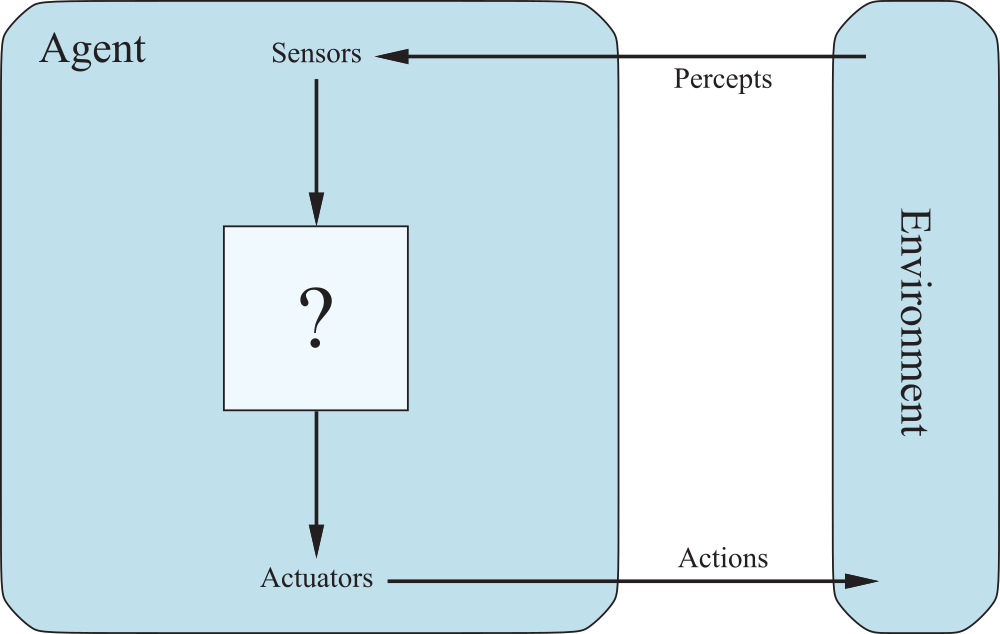
\includegraphics{Images/Chapter 1/agent-environment-schema.png}
    \caption{Schema of the interaction between an agent and the environment.}
    \source{Russel and Norvig, 2020}
    \label{fig:ch1-agentenvironmentschema}
\end{figure}
\begin{figure}[hbtp]
    \centering
    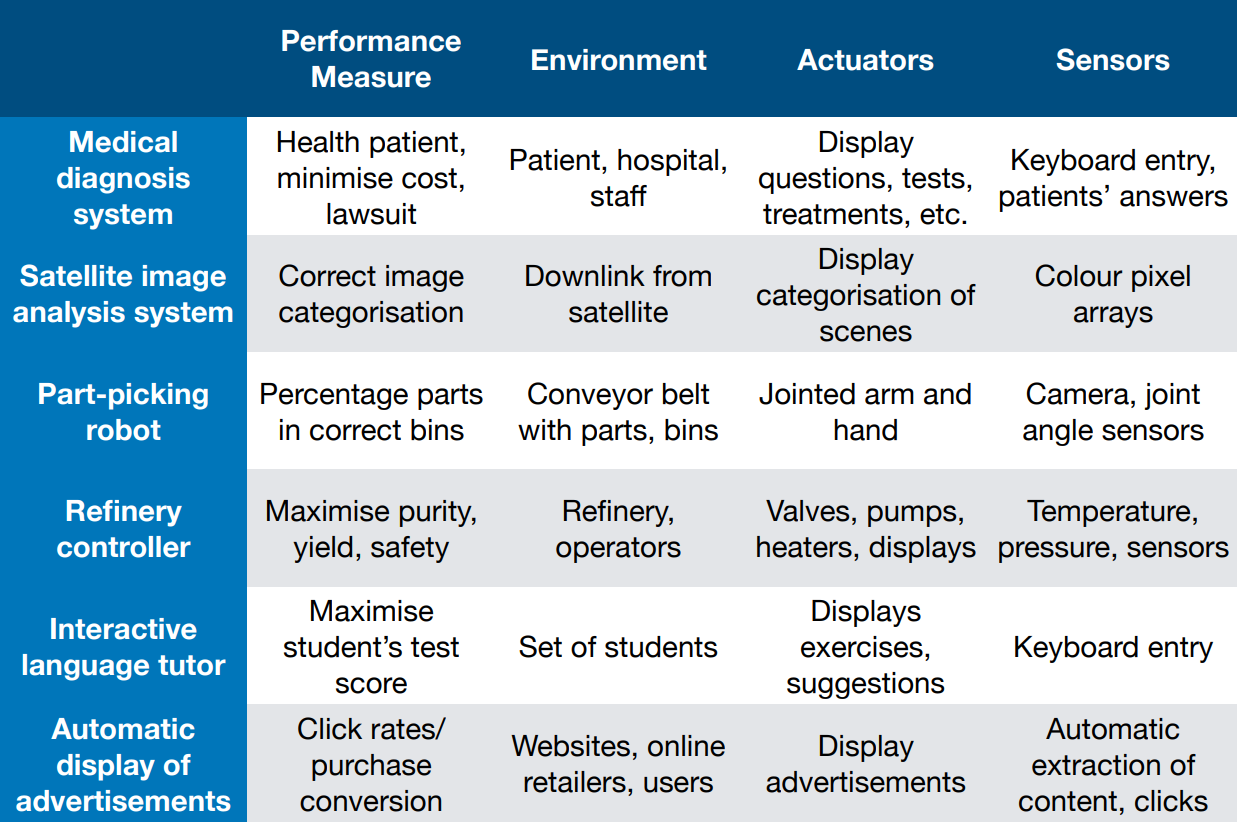
\includegraphics[width=\textwidth]{Images/Chapter 1/agents-type.png}
    \caption{Examples of agents and their characteristics.}
    \source{Prof. Mirco Musolesi}
    \label{fig:ch1-agentexamples}
\end{figure}

\section{Characteristics of the environments}
The environment in which our agent is situated may be of different types:

\begin{itemize}
    \item \textbf{Fully observable vs partially observable}: we may or may not be able to see the entire environment (e.g., there may be occlusions limiting our sight).
    \item \textbf{Deterministic vs stochastic}: the environment may be predictable (e.g., governed by the laws of Newtonian physics) or not (e.g., the environment may be subject to changes performed by another agent).
    \item \textbf{Episodic vs sequential}: the environment may be divided in “episodes” that have a beginning and an end (e.g., the levels of a game) or open-ended (e.g., a self-driving car that keeps on driving).
    \item \textbf{Static vs dynamic}: the environment may or may not change over time (an action that we take now could have a different result compared to when we took it in the past, e.g., certain agents with whom we collaborated in the past, may not do so anymore; driving in dry conditions is different compared to driving in the rain or in the snow; etc.).
    \item \textbf{Discrete vs continuous}: the environment may be represented by means of discrete or continuous values (e.g., a switch can be ON or OFF; the wind speed might be 14.6 km/h from N/E; etc.).
    \item \textbf{Single-agent or multi-agent}: there may be multiple agents in the environment, and we might want them to collaborate.
\end{itemize}

\section{A categorization of intelligent agents}
There are essentially four basic kinds of agents:

\begin{itemize}
    \item \textbf{Simple reflex agents}.
    \item \textbf{Model-based reflex agents}.
    \item \textbf{Goal-based agents}.
    \item \textbf{Utility-based agents}.
\end{itemize}

The behavior of these agents can be hard-wired, or it can be acquired, improved, and optimized through learning.

\subsection{Simple reflex agents}
Simple reflex agents (figure \ref{fig:ch1-simplereflexagent}) select actions on the basis of the current perceptions, ignoring the perception history. They are the most basic form of agents and are based on condition-action rules (also called \textbf{stimulus-response} rules, productions, or if-then rules).

\begin{figure}[hbt]
    \centering
    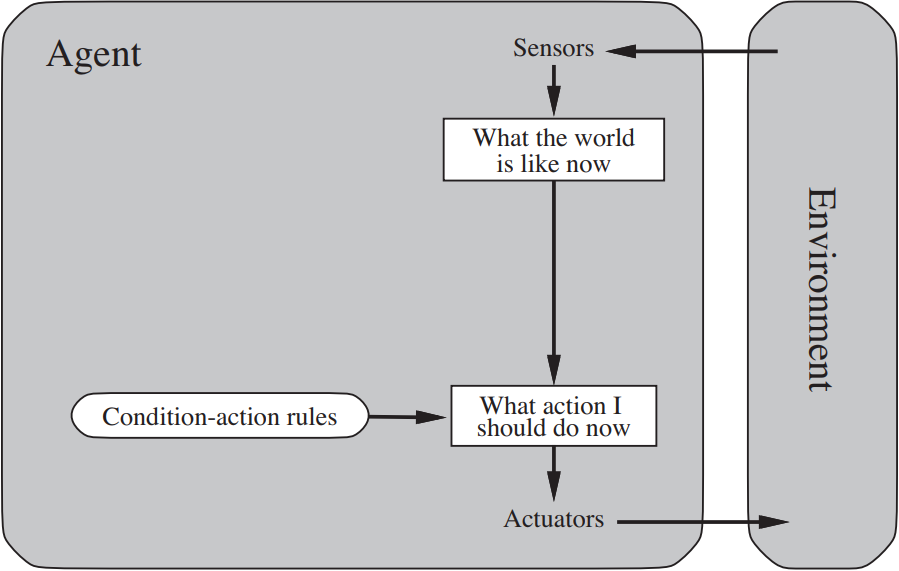
\includegraphics{Images/Chapter 1/simple-reflex-agents.png}
    \caption{Schema of a simple reflex agent.}
    \source{Russel and Norvig, 2020}
    \label{fig:ch1-simplereflexagent}
\end{figure}

\subsection{Model-based reflex agents}
Model-based agents (figure \ref{fig:ch1-modelbasedreflexagent}) keep an internal state and depend on two types of knowledge:

\begin{itemize}
    \item How the world evolves independently from the agent (e.g., the trajectory that a bullet/a stone follows when shot/thrown).
    \item How the actions of the agent affect the world (e.g., if I turn the wheel to the right, the car moves to the right).
\end{itemize}

The internal state is essentially used to keep track of what it is not possible to see/perceive at the current time. It depends on the perception history and, for this reason, it reflects at least some of the unobserved aspects of the current state.

\begin{figure}[hbtp]
    \centering
    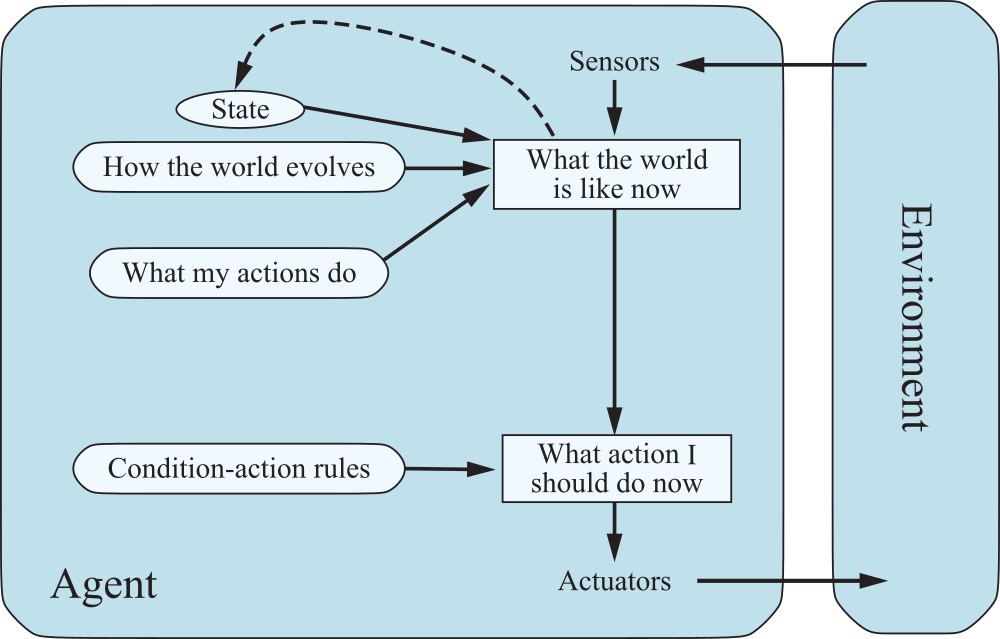
\includegraphics{Images/Chapter 1/model-based-reflex-agent.png}
    \caption{Schema of a model-based reflex agent.}
    \source{Russel and Norvig, 2020}
    \label{fig:ch1-modelbasedreflexagent}
\end{figure}

\subsection{(Model-based) Goal-based agents}
Goal-based agents (figure \ref{fig:ch1-goalbasedagent}) act in order to achieve their goals. If we can achieve the goal by carrying out a single action, goal-based action selection is straightforward; in the other cases, the agent needs to consider a long sequence of actions by means of search and planning.

\begin{figure}[hbtp]
    \centering
    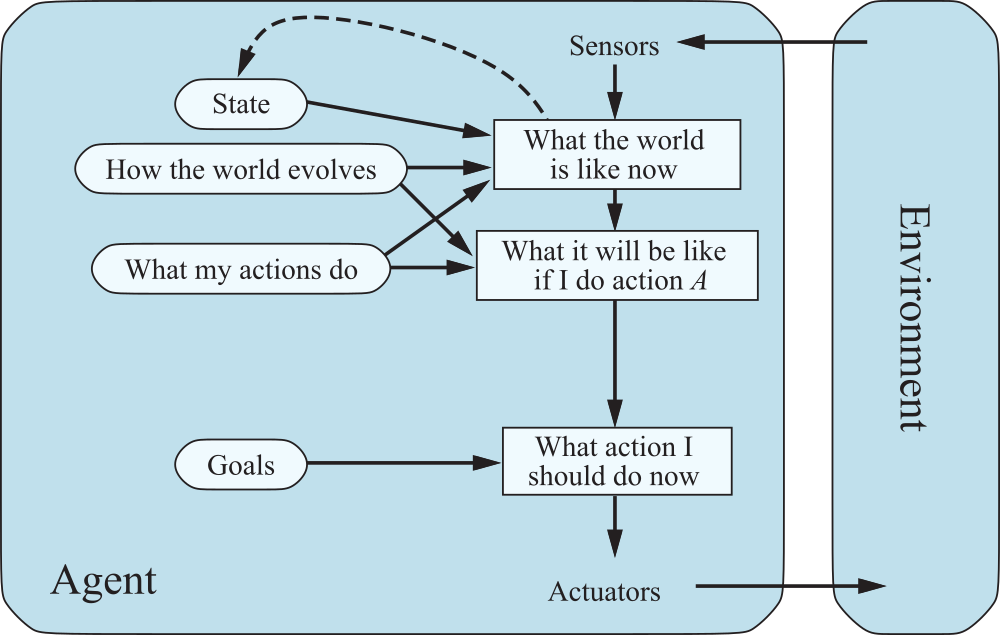
\includegraphics{Images/Chapter 1/goal-based-agent.png}
    \caption{Schema of a goal-based agent.}
    \source{Russel and Norvig, 2020}
    \label{fig:ch1-goalbasedagent}
\end{figure}

\subsection{(Model-based) Utility-based agents}
Goals are not sufficient to generate high-quality behavior in most environments, since there are usually states that are preferrable to others. In order to code this preference, we use utility functions that map a state (or a sequence of states) to a real number (e.g., we want to get to a destination by following the shortest or quickest path). (See figure \ref{fig:ch1-utilitybasedagent})

Note that how to model these preferences is one of the current unsolved and “hot” topics in the artificial intelligence field.

\begin{figure}[hbtp]
    \centering
    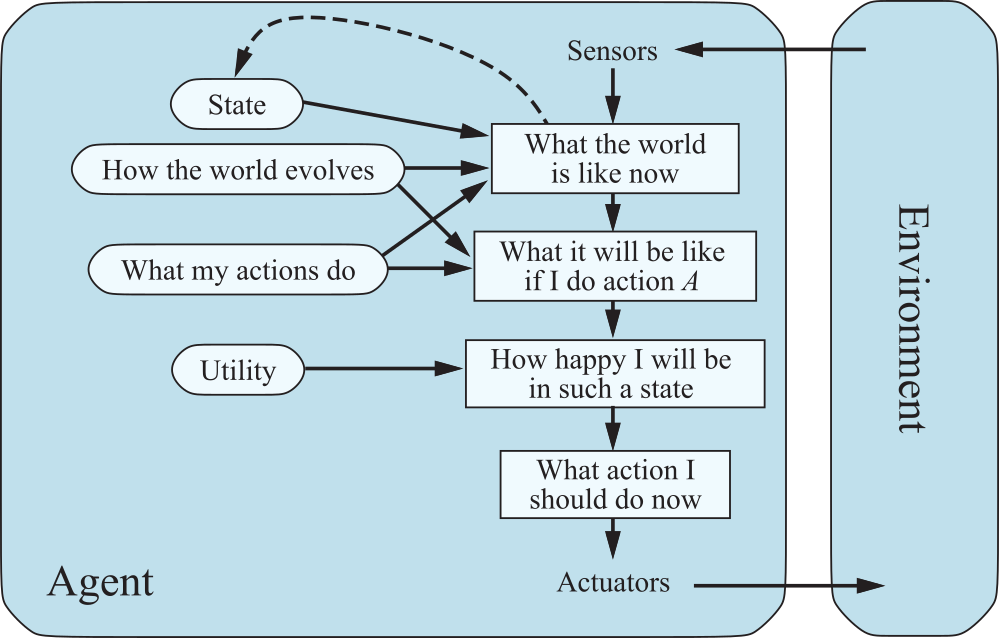
\includegraphics{Images/Chapter 1/utility-based-agent.png}
    \caption{Schema of a utility-based agent.}
    \source{Russel and Norvig, 2020}
    \label{fig:ch1-utilitybasedagent}
\end{figure}

To conclude this first introduction, let us quickly consider the topic of learning.

\section{Learning}
As we said before, the behavior of the agents can be pre-programmed (hard-wired, fixed) or it can be learned by means of a learning component. This component can be based on a model of the world and the gain towards a certain goal can be expressed through rewards. This behavior is at the basis of the type of learning that we will explore in detail in this course, called \textbf{reinforcement learning}. Following Herbert Simon’s definition of autonomous and adaptive systems, we will consider \textit{``machines that think, that learn and that create''}.
\chapter{Introduction to Reinforcement Learning}
The Merriam-Webster dictionary defines learning as the \textit{``modification of a behavioral tendency by experience''}\footnote{\url{https://www.merriam-webster.com/dictionary/learning}}. Interacting with the external world to learn, in fact, is an idea that is at the basis of nearly all theories of learning and intelligence. In the artificial intelligence world, this approach is leveraged with success in reinforcement learning.

\textbf{Reinforcement learning is learning what to do and how to map situations to actions, so as to maximize a numerical reward} (it is goal-directed learning from interaction). The learner is not told which actions to take, but instead it must discover which actions yield the most reward by trying them out. In the most interesting and challenging cases, actions may affect not only the immediate reward but also the next situation and, through that, all subsequent rewards. These two characteristics (trial-and-error search and delayed reward) are the two most important distinguishing features of reinforcement learning.

We will now introduce finite Markov decision processes, a mathematical framework that we are going to use.

\section{Finite Markov Decision Processes}
Markov Decision Processes (MDPs) are a mathematically idealized formulation of reinforcement learning for which precise theoretical statements can be made. They provide a mathematical framework for modeling decision making in situations where outcomes are partly random and partly under the control of a decision maker\footnote{See \url{https://en.wikipedia.org/wiki/Markov_decision_process}}.

At each time step $t$, the process is in some state $s$, and the decision maker may choose an action $a$ that is available in state $s$. The process responds at the next time step by randomly moving into a new state $s'$, and giving the decision maker a corresponding reward $R_a(s,s')$. The probability that the process moves into its new state $s'$ is influenced by the chosen action. Specifically, it is given by the state transition function $P_a(s,s')$. Thus, the next state $s'$ depends on the current state $s$ and the decision maker's action $a$. But \textbf{given $\boldsymbol{s}$ and $\boldsymbol{a}$, it is conditionally independent of all previous states and actions}; in other words, the state transitions of an MDP satisfy the Markov property \textit{(memoryless property of a stochastic process)}.

\begin{figure}[hbt]
    \centering
    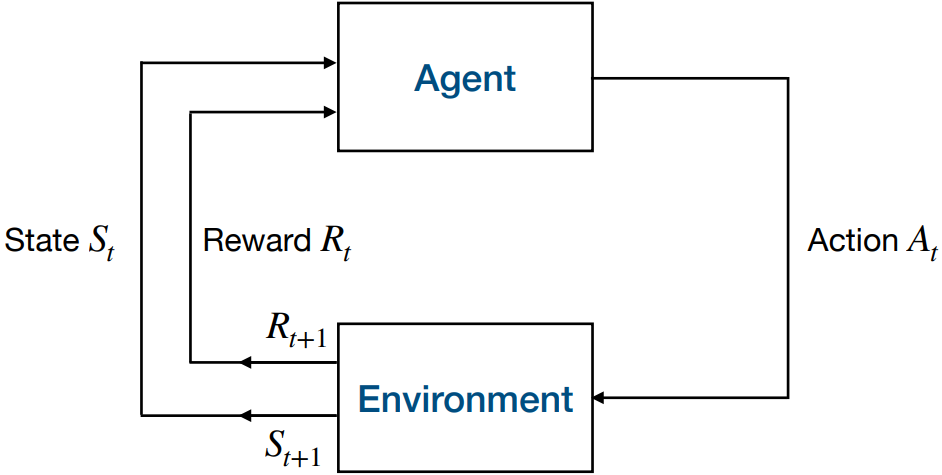
\includegraphics[width=\textwidth]{Images/Chapter 2/mdp.png}
    \caption{Schema of a Markov Decision Process.}
    \source{Prof. Mirco Musolesi}
    \label{fig:ch2-mdp}
\end{figure}

\section{Rewards and expected returns}
Informally, the agent’s goal is to maximize the \textbf{total amount} of rewards it receives (note how the agent should not maximize the immediate reward, but the cumulative reward). We can formalize this with the \textbf{``reward hypothesis''}: \textit{``That all of what we mean by goals and purposes can be well thought of as the maximization of the expected value of the cumulative sum of a received scalar signal (called reward)''}.

We will now try to conceptualize the idea of \textbf{cumulative rewards} more formally by means of the notion of \textbf{expected return} $\boldsymbol{G_t}$. To do so, we first need to distinguish between two cases:

\begin{itemize}
    \item \textbf{Episodic tasks}, in which we can identify a final step of the sequence of rewards (i.e., in which the interaction between the agent and the environment can be broken into sub-sequences called \textbf{episodes}, such as playing a game, repeated tasks, etc.). Each episode ends in a terminal state after $T$ steps, followed by a reset to a standard starting state or to a sample of a distribution of starting states (the next episode will be completely independent from the previous one).
    \item \textbf{Continuous tasks}, in which the agent-environment interaction does not break naturally into identifiable episodes, but goes on continually without limit (e.g., an ongoing monitoring of a process).
\end{itemize}

The expected return $G_t$ associated to the selection of an action $A_t$, assuming that the agent receives over time a sequence of rewards $R_{t+1}, R_{t+2}, R_{t+3}, ...$ is defined as:

\begin{itemize}
    \item The \textbf{sum of future rewards} in the case of \textbf{episodic tasks}:
    \begin{equation}
        G_t \doteq R_{t+1} + R_{t+2} + R_{t+3} + ... + R_T
        \label{eq:ch2-expectedreturn-episodic}
    \end{equation}
    \item The \textbf{discounted sum of future rewards} in the case of \textbf{continuing tasks}:
    \begin{equation}
        G_t \doteq R_{t+1} + \gamma R_{t+2} + \gamma^2 R_{t+3} + ... = \sum_{k=0}^{\infty} \gamma^k R_{t+k+1}
        \label{eq:ch2-expectedreturn-continuous}
    \end{equation}
\end{itemize}

Where $\gamma$ is the \textbf{discount rate}, with $0 \le \gamma \le 1$. The discount rate is used to give more importance to the rewards that are closer to us in time; this is particularly useful in dynamic environments. The definition of expected return that we used for episodic tasks would in fact be problematic for continuing tasks: the expected return would be equal to $\infty$ (in the limit of an infinite number of time steps) in some cases, such as when the reward is equal to $1$ at each time step. The discount rate then determines the ``present value of future rewards'' (how much future rewards mean to us at the current time): a reward received $k$ time steps in the future is worth $\gamma^{k-1}$ of what it would be worth if it were received immediately.

Returns at successive time steps are related to each other as follows:

\begin{equation*}
    \begin{split}
        G_t & \doteq R_{t+1} + \gamma R_{t+2} + \gamma^2 R_{t+3} + \gamma^3 R_{t+4} + ... \\
        & = R_{t+1} + \gamma \left( R_{t+2} + \gamma R_{t+3} + \gamma^2 R_{t+4} + ... \right) \\
        & = R_{t+1} + \gamma G_{t+1} \\
    \end{split}
\end{equation*}

\section{Policies and value functions}
Almost all reinforcement learning algorithms involve estimating value functions, i.e., functions of states (or of state-action pairs) that estimate how good it is for the agent to be in a given state (or how good it is to perform a given action in a given state). The notion of ``how good'' here is defined in terms of future rewards that can be expected, or, to be precise, in terms of expected return.

A \textbf{policy} is used to model how the agent will behave based on the previous experience and the rewards an agent received in the past (and, consequently, the expected returns). Formally, a policy is a mapping from states to probabilities of taking each possible action (the probability of taking a certain action in a certain state). If the agent is following the policy $\pi$ at time $t$, then $\pi (a \vert s)$ is the probability that $A_t=a$ if $S_t=s$.

\textbf{The value function of a state $\boldsymbol{s}$ under a policy $\boldsymbol{\pi}$}, denoted $v_\pi (s)$, is the expected return when starting in $s$ and following $\pi$ thereafter (the expected return I can have in the future state, considering all the actions I might take from there). For Markov Decision Processes, we can define \textbf{the state-value function} $\boldsymbol{v_\pi}$ for the policy $\pi$ formally as:

\begin{equation}
    v_\pi(s) \doteq \mathbb{E}_\pi \left[ G_t  \ \vert \  S_t = s \right] = \mathbb{E}_\pi \left[ \sum_{k=0}^{\infty}  \gamma^k R_{t+k+1} \  \middle\vert \  S_t = s, A_t = a \right] \quad \forall s \in \mathcal{S}
    \label{eq:ch2-statevaluefunction}
\end{equation}

Where $\mathbb{E}_\pi [\cdot]$ denotes the expected value of a random variable given that the agent follows $\pi$ and $t$ is any time step. Note that the value of the terminal state, if any, is always $0$. The formula above denotes a weighted average of the expected value (it is averaged because the values depend on the probability of a certain action being taken, which is a fraction).

Similar to what we just did, we can define \textbf{the action-value function}, i.e., the value of taking an action $a$ in the state $s$ under a policy $\pi$, denoted $\boldsymbol{q_\pi (s,a)}$, as the expected return starting from $s$, taking the action $a$, and following the policy $\pi$ thereafter:

\begin{equation}
    q_\pi(s,a) \doteq \mathbb{E}_\pi \left[ G_t \  \vert \  S_t = s, A_t = a \right] = \mathbb{E}_\pi \left[ \sum_{k=0}^{\infty} \gamma^k R_{t+k+1} \  \middle\vert \ S_t = s, A_t = a \right]
    \label{eq:ch2-actionvaluefunction}
\end{equation}

\section{Choosing the rewards}
When we model a real system as a reinforcement learning problem, the most difficult task is selecting the right rewards. Typically, we use negative values for actions that do not help us in reaching our goal, and positive if they do (it is also possible using 0 as a value for actions that do not help us). An alternative is to set the values of the rewards to a negative number until we reach our goal (using 0 as the value when we reach it).

When choosing the rewards, it is very important that \textbf{we should not ``reward'' the intermediate steps or the single actions}. The agent, in fact, always learns to maximize its reward. If we want it to do something for us, we must provide rewards to it in such a way that in maximizing them the agent will also achieve our goals. It is thus critical that the rewards we set up truly indicate what we want accomplished. If we were to give importance to certain sub-goals, the agent might find a way to achieve them without achieving the real goal (e.g., taking the opponent's pieces while playing chess but losing the game). Note that the reward signal is our way of communicating to the agent \textit{what} we want achieved, not \textit{how} (a better place for imparting this kind of prior knowledge would be the initial policy or the initial value function).

Giving rewards to the agent could be a challenging task, as we will see from the two examples that follow. Let us first imagine that we want to create an agent that completes a maze in the least time possible: we could give a reward of -1 for every step it takes inside the maze and 0 for reaching the exit. This could work even if we assume that we only have one episode to base our rewards on. There are situations, though, in which we need additional information to quantify how good an action is for us, like in a game of chess, where we can only assign the rewards at the end of the game (e.g., assigning 1 to every step if we won, -1 if we lost). This is usually called \textbf{credit assignment problem} (i.e., the problem of assigning a reward to each step) and a discussion on it can be found in Marvin Minsky’s ``Steps Towards Artificial Intelligence'' paper \cite{4066245}.

We now need to think about how we can solve this problem and estimate the value functions $v_\pi$ and $q_\pi$. If the behavior of the Markov Decision Process is known (i.e., the transition probabilities between all the states are known), we could do so by considering all the possible moves, although this poses strict requirements in terms of prior knowledge and system complexity. A more general option is to estimate them through experience: if an agent follows policy $\pi$ and maintains an average, for each state encountered, of the actual returns that have followed that state, then the average will converge asymptotically to the state’s value, $v_\pi(s)$, as the number of times that that state is encountered approaches infinity (these methods are referred to as \textbf{Monte Carlo methods} because they involve averaging over many random samples of actual returns). This option is still problematic when it comes to very large number of states, though, as it would involve keeping separate averages for each state individually. In those cases, instead, we will maintain $v_\pi$ and $q_\pi$ as parametrized functions, with fewer parameters than the number of states, using approximators such as artificial neural networks.

\section{Optimal policies and optimal value functions}
Solving a reinforcement learning task is roughly equivalent to finding a policy that maximizes the reward in the long run. In finite Markov Decision Processes, there is always at least one policy $\pi$ that is better than (or equal to) all the other policies, meaning that its expected return is greater than (or equal to) that of a different policy $\pi'$ for all states. More formally:

\begin{equation*}
    \pi \ge \pi' \text{ if and only if } v_\pi(s) \ge v_{\pi'} (s) \quad \forall s \in \mathcal{S}
\end{equation*}

Although there may be more than one, we denote all the optimal policies with $\pi_*$. They share the same state-value function, called the \textbf{optimal state-value function}, denoted $v_*$ and defined as:

\begin{equation}
    v_*(s) \doteq \max_\pi v_\pi(s) \quad \forall s \in \mathcal{S}
    \label{eq:ch2-optimalstatevaluefunction}
\end{equation}

This means that, given a state and the value function, the optimal policy is the one that gives us the maximum reward. The same goes for the \textbf{optimal action-value function}, denoted $q_*$ and defined as:

\begin{equation}
    q_*(s,a) \doteq \max_\pi q_\pi(s,a) \quad \forall s \in \mathcal{S}, a \in \mathcal{A}(s)
    \label{eq:ch2-optimalactionvaluefunction}
\end{equation}

For the state-action pair $(s,a)$, this function gives the expected return for taking the action $a$ in the state $s$ and thereafter following an optimal policy. Thus, we can write $q_*$ in terms of $v_*$ as follows:

\begin{equation*}
    q_*(s,a) = \mathbb{E}_{\pi} \left[ R_{t+1} + \gamma v_* S_{t+1} \  \middle\vert \ S_t = s, A_t = a \right]
\end{equation*}

\section{Optimality and approximation}
\subsection{Bellman equation}
What we are doing is closely related to the issues of automatic control: we both want to have knowledge and control over the evolution of a system.

For any policy $\pi$ and any state $s$, the following consistency condition holds between the value of $s$ and the value of its possible successor states:

\begin{equation}
    \begin{split}
        v_\pi(s) & \doteq \mathbb{E}_\pi \left[ G_t \ \vert \ S_t = s \right] \\
        & = \mathbb{E}_\pi \left[ R_{t+1} + \gamma G_{t+1} \ \vert \ S_t = s \right] \\
        & = \sum_{a} \pi(a \vert s) \sum_{s'} \sum_{r} p(s',r \ \vert \ s,a) \Big[ r + \gamma \mathbb{E}_\pi \left[ G_{t+1} \ \vert \ S_{t+1} = s' \right] \Big] \\
        & = \sum_{a} \pi (a \vert s) \sum_{s', r} p(s', r \ \vert \ s,a) \Big[ r + \gamma v_\pi(s') \Big], \quad \forall s \in \mathcal{S}
    \end{split}
    \label{eq:ch2-bellmanequation}
\end{equation}

What we have in the end is known as the \textbf{Bellman equation} for $v_\pi$ and it states that the value of the start state must equal the (discounted) value of the expected next state, plus the reward expected along the way.

\subsection{Bellman optimality equation}
We can re-write the Bellman equation under the optimal policy, obtaining what is known as the \textbf{Bellman optimality equation}:

\begin{equation}
    \begin{split}
        q_*(s,a) & = \mathbb{E}_{\pi} \left[ R_{t+1} + \gamma \max_{a'} q_* (S_{t+1}, a') \ \middle\vert \ S_t = s, A_t = a \right] \\
        & = \sum_{s', r} p(s',r \ \vert \ s,a) \left[ r + \gamma \max_{a'} q_*(s',a') \right]
    \end{split}
    \label{eq:ch2-bellmanoptimalityequation}
\end{equation}

Intuitively, the Bellman optimality equation must equal the expected return for the best action from that state. 

The Bellman optimality equation is actually a system of equations, one for each state, so if there are $n$ states, then there are $n$ equations in $n$ unknowns. If the dynamics $p$ of the environments are known, then in principle one can solve this system of equation for $v_*$. Once we have $v_*$ (or $q_*$), the actions that select the highest value for them in each state will then be the optimal actions. Another way of saying this is that any policy that is \textbf{greedy} with respect to the optimal evaluation function is an optimal policy. As a reminder, the term \textit{greedy} is used in computer science to describe any search or decision procedure that selects alternatives based only on local or immediate considerations, without considering the possibility that such a selection may prevent future access to even better alternatives. This is not an issue in the case of Markov Decision Processes, though, as they depend only on the current state: \textbf{a greedy policy is then optimal both in the short and in the long-term}.

As we were hinting at earlier, it may not always be possible to solve the Bellman optimality equations, both due to the huge number of states (and equations) involved in non-trivial problems and because the state may not be fully observable, or we may not be able to know its dynamics.

% Bibliography
\clearpage
\printbibliography

\end{document}
